The results of our experiments for the %success 
prediction of online crowdfunding campaign success is presented in Table \ref{tab:results}. Our models with knowledge-infused representations (\#6-17) provided overall better performance compared to the baseline models (\#1-5). The best performance was achieved with Resnet152 and RoBERTa with the TransE KG embeddings with 0.95, 0.91, and 0.92, precision, recall, and F1-score, respectively. The lowest performance came from the MDL-TIM model (\#4) while the two baseline models, ViT/RoBERTa (\#3) and BLIP-only (\#5), were much better. However, knowledge-infused models consistently performed better. In terms of AUC, our best knowledge-infused model (\#12) outperforms other models with 94\%, indicating a higher true positive rate and a lower false positive rate. The outperformance of our model in AUC also signals potential improvement in the fairness of the model, warranting future work on the fairness assessment of knowledge-infused models. 
% \textcolor{red} {Where is the promised error analysis?  Where is the potential explanation?}

Following up on our research questions; upon these results, we have observed that incorporating external knowledge in learning multimodal representations improves the contextual congruence of the representations of multimodal content, unveiling subtle cross-modal semantic relationships (RQ1). When we use these knowledge-infused representations in our downstream task, prediction of the success of multimodal marketing campaigns, it provides more consistent and reliable predictive performance (RQ2).

\begin{figure}[htb!]
  \centering
  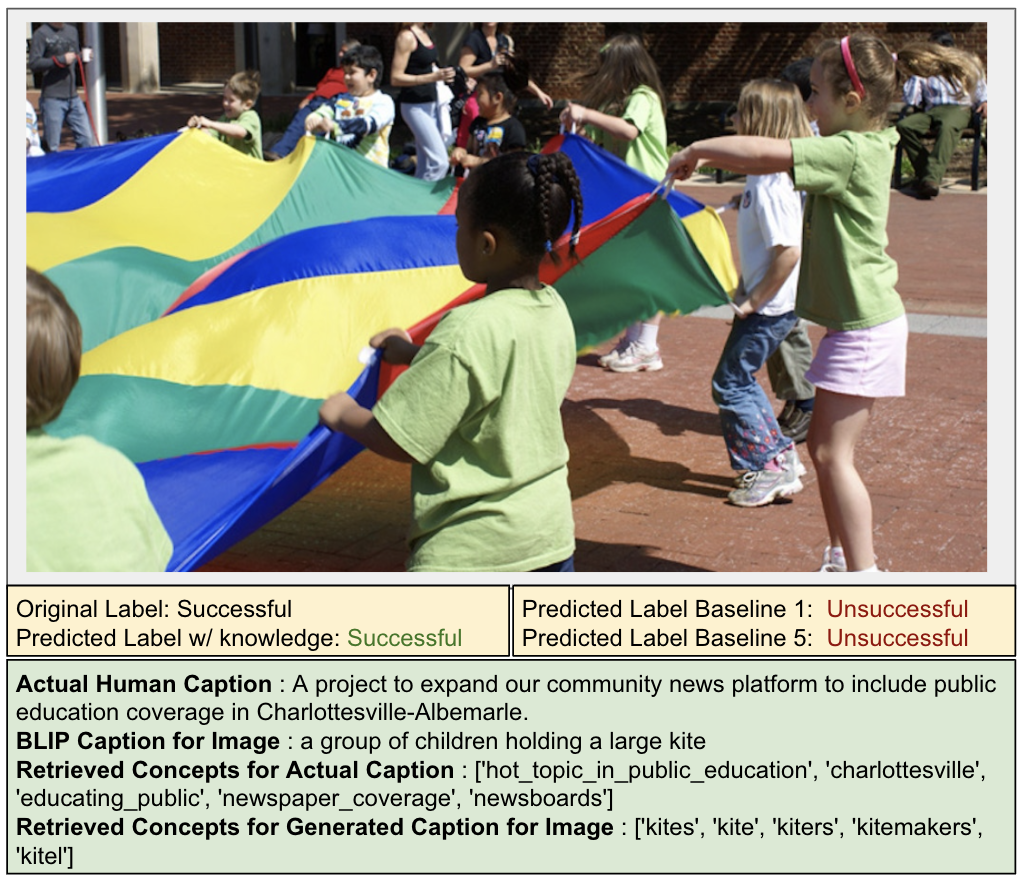
\includegraphics[width=8.5cm]{Figures/erroranalysis/error-analysis-sucess-community-project2.png}
\vspace{-1.5em}
\caption{The yellow box contains the model prediction with knowledge and two baseline models. The green box shows the actual caption, BLIP caption, and retrieved concepts for each modality.}
\vspace{-1em}
\label{fig:error-analysis-kites-educating-public}
\end{figure} 

\subsection{Error Analysis}
Overall, this analysis aims to explore the contribution of contextual congruence utilizing KGs in multimodal models, as well as limitations compared to baseline models. Hence, we examined a small number of data points where models with knowledge predicted correctly and incorrectly. We make the following observations:
%We delve into various scenarios where the improved model surpasses the baseline's shortcomings and identifies cases where the improved model falters due to the incorporation of noisy knowledge retrieval. By understanding these dynamics, we gain insights into the strengths and weaknesses of the enhanced model, contributing to a more nuanced understanding of its performance. Baseline models are the initial benchmark against which advancements are evaluated. However, in capturing the multimodal semantic relationships, these models display significant limitations, often struggling with complex patterns and nuanced relationships within the data. The improved model builds upon these weaknesses, incorporating commonsense knowledge from Conceptnet to overcome the baseline's shortcomings. While the improved model generally outperforms the baseline, its reliance on noisy knowledge retrieval presents its own set of challenges.

\noindent \textbf{Erroneous Omissions in Baseline Models.}  In Figure \ref{fig:error-analysis-kites-educating-public}, %it could be seen how 
the model with knowledge captures the important concepts or events that connect the image and text to prevent incorrect predictions, misclassifications, and an overall lack of precision. For instance, the baseline models can possibly recognize only objects and shallow details, while additional knowledge and relationships in between provide deeper context into the meaning of the content. The concept \textit{'hot\_topic\_in\_public\_education'} showcases students as \textit{‘kitemakers’}, \textit{'educating\_public'}  to support innovative teaching methods by \textit{'newspaper\_coverage'}. Such additional richer contextual knowledge helps the model to make better inferences for the meaning of content. 
%Consequently, the improved model excels in scenarios where the baseline faltered. It showcases better accuracy, improved generalization, and higher predictive power. Notably, these could be seen 
Similar limitations for baselines and advantages of knowledge infusion appear in  Figures \ref{fig:error-analysis-poetry-graffiti}, \ref{fig:error-analysis-woofer-error-analysis} and \ref{fig:error-analysis-sucess-poet}. 

%[Noisy Knowledge Retrieval and Its Impact:] 
\noindent \textbf{Erroneous Commissions in the Improved Models.}  The incorporation of noisy knowledge retrieval mechanisms into the improved model introduces a new set of challenges. In some cases, the model retrieves information that is either irrelevant or contradictory to the context.
%, leading to flawed predictions. 
This phenomenon is particularly prominent when the BLIP model fails to capture the main entities in the context of the image. 
%While the improved model demonstrates impressive performance, it is not immune to the issues introduced by noisy knowledge retrieval. Instances where the model fails due to such noise could be seen in 
(see Figure \ref{fig:error-analysis-failure-mens-mental-health}) where the campaign talks about how abuse and mental health issues suffered by men are often neglected.
%which can be seen in t
The campaign advertisement depicts men in a smaller size and women in a larger size, symbolizing the disproportionate attention given to men’s issues compared to women's. 
%By highlighting this disparity, but since 
As the knowledge retrieved for the image is from ConceptNet through the BLIP caption, many noisy concepts get infused, such as \textit{'front\_wall'}, \textit{'wall\_placement'}, \textit{'front\_walls'}, \textit{'recolor\_wall'}. %it is difficult to understand the context.
This analysis highlights the trade-off between performance enhancement through complex modeling and the susceptibility to noisy knowledge. While the recall improves at the expense of precision with knowledge-infused models, in the case of any misclassifications, the model may predict if a marketing campaign will be successful which may lead to possible financial loss.

\noindent \textbf{Social Impact.} Understanding (and thereby predicting) multimodal persuasiveness has extensive application. These are both benign, as in purchasing products or services, or malicious where prediction is a paramount tool for ensuring safety. In this regard, we note high recall (i.e., low false negatives) without reducing precision (i.e., low false positives), along with higher AUC, warranting further investigation for improvements in fairness using our approach. This distribution of error bears on detection efficiency of critical importance when the cost of error is high and detection requires manual follow-up. While we demonstrate such enhancement for effective multimodal marketing, a similar approach will be necessary for other context-sensitive social and behavioral problems including toxicity and extremism, among others. Further, there are still unknown implications of these AI-enabled technologies for individuals and communities, specifically, underrepresented groups in society. This work specifically provides potential avenues to address social biases, inadvertently encoded in large foundation models (e.g., LLMs, LVMs, VLMs) using a framework that incorporates external knowledge in learning, for future work.

%The insights gained from this analysis offer guidance for future model refinement and robust knowledge infusion techniques

%In conclusion, this error analysis sheds light on the contrasting performances of baseline and improved models within the context of preidcing the success of Multimodal marketing campaign, While the improved model exhibits superior predictive capabilities, it is crucial to remain mindful of the challenges posed by noisy knowledge retrieval. Through a balanced approach, the field can continue to make strides towards more accurate and robust models.



\begin{figure}
  \centering
  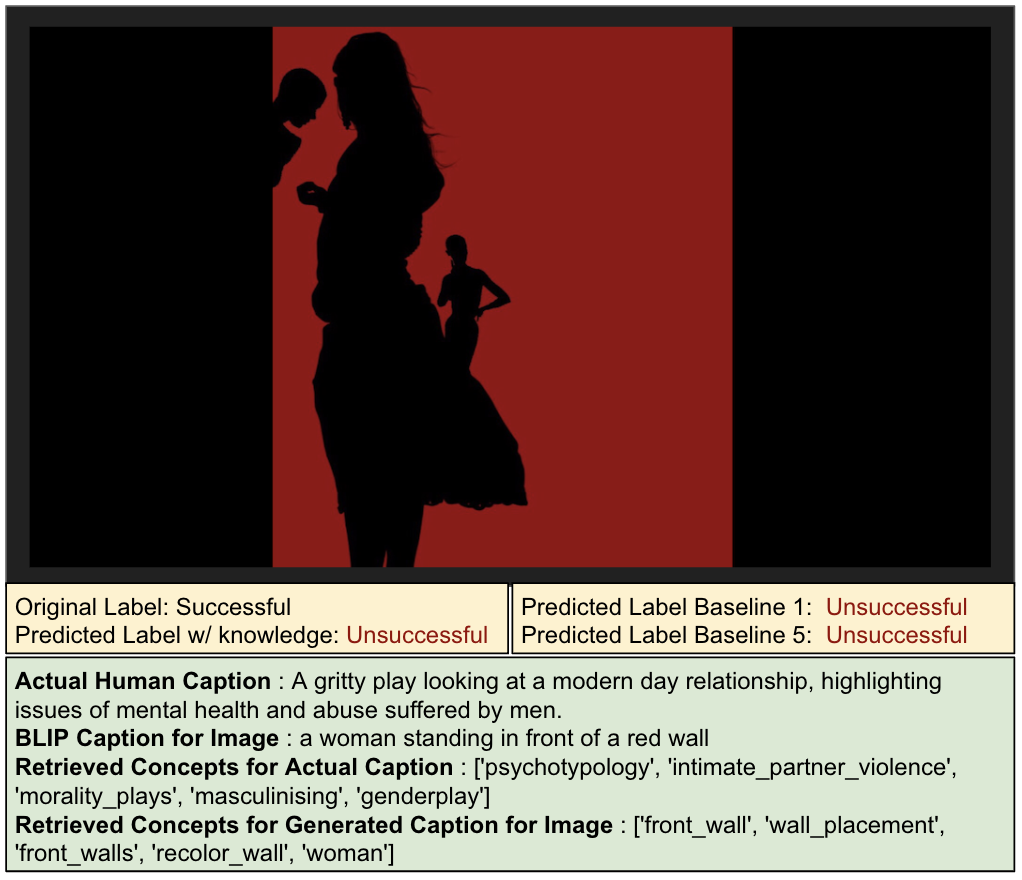
\includegraphics[width=8.5cm]{Figures/erroranalysis/error-analysis-failure-mens-mental-health2.png}
\vspace{-1.5em}
\caption{In this example, the model with knowledge could not also predicted accurate label along with other baseline models.}
% \textbf{Explanation:} The campaign talks about how abuse and mental health issues suffered by men are often neglected which can be seen in the campaign advertisement, which depicts men in a smaller size and women in a larger size, symbolizing the disproportionate attention given to women’s issues compared to men's. By highlighting this disparity, the campaign aims to raise awareness about the importance of addressing and supporting men's mental health struggles, ultimately advocating for equal treatment and resources for all genders.
% Since the knowledge retrieved for the image has lot of noisy concepts which get infused, such as 'front\_wall', 'wall\_placement', 'front\_walls', 'recolor\_wall', it is difficult to understand the context.}
\vspace{-1.5em}
\label{fig:error-analysis-failure-mens-mental-health}
\end{figure} 


\noindent \textbf{Limitations.} Utilizing KGs to improve contextual congruence across various modalities shows great potential, particularly in marketing. This approach can be adaptable to various fields, and we acknowledge that further research is necessary to validate its effectiveness beyond marketing. We also recognize that the knowledge-infused approach does encounter challenges with noisy triples from the KG, underscoring the need for enhanced robustness. While the approach is applied to marketing, generally a benign domain, it can be misused with malicious intent such as creating highly persuasive and targeted misinformation campaigns. Therefore, we emphasize the need to follow ethical guidelines and responsible use of these novel approaches to prevent  negative outcomes. The data used in this study may contain possible artifacts based on the "country" attribute, which we leave to address in future work. We anonymized our dataset to omit any identifiable information. We limited our experiments to the open-source models due to the prohibitively high computational costs of commercial models for academic research. 